\chapter{Simulation von Streubildern}
Das Problem der Berechnung synthetischer Streubilder besitzt verschiedene Lösungsansätze. Neben den verbreiteten Methoden \textit{DDA} und \textit{FDTD}, die in allen Raumrichtungen Berechnungspunkte in einem Abstand deutlich geringer als die Wellenlänge benötigen und der 3d-Fouriertransformierten, die zwar mit weniger Punkten noch valide Ergebnisse liefern kann, bei der jedoch ebenfalls der Berechnungsaufwand die möglichen Objekte deren Streubilder berechnet werden soll limitiert, existieren verschiedene Ansätze. 

\section{Mie Streuung}
Die Mie-Theorie bietet eine analytische Lösung der Streuung an einer Kugel in Form einer unendlichen Reihe basierend auf einer Lösung der Grenzbedingungen für elektromagnetische Wellen \cite{bohren2008}. Die unendliche Reihe lässt sich näherungsweise numerisch berechnen (Details siehe \fref{app:mie}).
Eine vektorisierte Version dieser Berechnung liegt in der auf Mätzler \cite{maetzler2002} basierenden Matlab Funktionen \texttt{simulation/mie.m} für winkelabhängige Radialprofile sowie \texttt{simulation/mie\_scatter.m} für Streubilder vor und dient der Verifizierung der Simulationsverfahren.

\section{Projektions- und Rayleigh-Gans-Näherung}
	
Um dreidimensionalen Streuobjekte durch zweidimensionale Blenden zu nähern, lässt sich die Projektion ihrer Dichteverteilung auf eine Ebene direkt hinter ihnen betrachten. In Näherung verhält sich eine elektromagnetische Welle nach Durchlaufen des Objektes gleich wie nach Durchlaufen einer Blende mit dieser durch Projektion gewonnenen Absorption und Refraktion, sodass in Fraunhofer-Fernfeldnäherung das Streubild durch die Fouriertransformierte der Projektion genähert werden kann.
	
Für eine kreisförmige Blende existiert eine analytische Darstellung der Fouriertransformation in Form der sogenannten Airy-Scheibe und das Streubild eines Objektes mit kreisförmiger Projektion lässt sich somit mittels der Besselfunktion 1. Ordnung $J_n$ als
\begin{equation}
	I(\theta) \propto \left ( \frac{2 J_1(kr \sin \theta)}{kr \sin \theta} \right )^2 
\end{equation}
nähern\cite{born1980}. Für nicht kreisförmige Projektionen der Dichte lässt sich die Fouriertransformation diskret numerisch auswerten.
Eine weitere gebräuchliche Näherung für kugelförmige Objekte ist die Rayleigh-Gans Näherung (gültig für kleine Radien und Brechzahlen nahe Vakuum). In dieser nimmt die Intensität die Form
\begin{equation}
	I(\theta)\propto\left ( \frac{j_1(2kr\sin(\theta/2))}{2kr\sin(\theta/2)} \right )^2 
\end{equation}
mit der sphärischen Besselfunktion $j_n$ an \cite{bohren2008}. 


\section{Multislice Fourier Transformation}
Nach \fref{eq:born} gilt in der ersten Bornschen Näherung für die Amplitude der gestreuten Welle
\begin{equation}
	\phi\propto\int \delta\eta(\vec{r}) e^{-i\vec{q}\cdot \vec{r}} \dif \vec{r}
\end{equation}
Wird das Skalarprodukt $\vec{q}\cdot \vec{r}=xq_x+yq_y+zq_z$ ausgeschrieben und die Integration über $x$ und $y$ als zweidimensionale Fouriertransformation interpretiert
\begin{equation}
	\phi\propto\int \mathscr{F}\left[\delta\eta\right](q_x,q_y,z) e^{-zq_z} \dif z \, ,
\end{equation}

so lässt sich das Integral in z-Richtung als Summe interpretieren sofern sich $q_z$ als $q_z=q_\parallel(k,q_\perp)$ ausdrücken lässt.
	
Aufgrund der Impulserhaltung muss $k_{ein}^2=k_{aus}^2=k^2$ gelten. Nach Abbildung \fref{fig:msft} ist
\begin{align}
	k^2=(k-q_\parallel)^2+q_{\perp}^2                  
	\Leftrightarrow q_\parallel=k-\sqrt{k^2-q_\perp^2} 
\end{align}
Somit
\begin{equation}
	\label{eq:msft}
	\phi\approx\sum_n{\mathscr{F}\left[\delta\eta\right] e^{-in\delta_z\left(k-\sqrt{k^2-q_\perp^2}\right) }}
\end{equation}

\begin{figure}
	\centering
	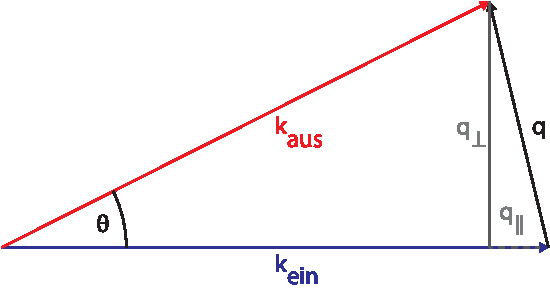
\includegraphics[width=0.5\textwidth]{images/msft.pdf}
	\caption[Vektoren bei MSFT]{Skizze zur Bezeichnung der Vektoren. $k_{ein}$ und $k_{aus}$ bezeichnen den Wellenvektor der einfallenden bzw. ausfallenden Welle mit dem dazwischenliegenden Winkel $\theta$. $q$ bezeichnet den Streuvektor mit einer zu $k_{ein}$ parallelen ($q_{||}$) und einer senkrechten ($q_\perp$) Komponente.}
	\label{fig:msft}
\end{figure} 

\fref{eq:msft} beschreibt einen Algorithmus um das Streubild eines dreidimensionalen Objektes im Fernfeld in der ersten Bornschen Näherung zu berechnen. Diese Methode wird als \textit{Multislice Fourier Transformation} \textit{MSFT} bezeichnet \cite{barke2015}. 
Bei dieser Methode wird Mehrfachstreuung vollständig ignoriert. Durch nachträgliches Einführen eines zusätzlichen Faktors, der die Absorption und Phasenänderung der Welle beim Durchlaufen des Objektes beschreibt, ließe sich nachträglich eine grobe Näherung für Absorptionseffekte einführen, die in einigen Fällen die subjektive Qualität der Simulation verbessern kann \cite{barke2015}. Da diese zum Einen jedoch nicht konsistent zur Herleitung der Methode ist und somit ihre Gültigkeit nicht abgeschätzt werden kann, zum anderen sie nicht allgemein die Güte der Simulation verbessert, ist im Weiteren mit \textit{MSFT} die Methode ohne diese Korrektur bezeichnet.
Eine Implementation des MSFT-Algorithmus mit optionaler Absorptionskorrektur liegt in \texttt{simulation/msft.m} vor. 

\section{Multislice Propagation}
Ein alternatives Verfahren zur Simulation von Streubildern ist in der Literatur als \textit{Multislice} oder \textit{Beam Propagation} bekannt \cite{hare1994,cowley1957}. Bei diesem Verfahren wird zunächst die Szene (ein definierter Raum in dem sich alle Objekte deren gemeinsames Streubild berechnet werden soll) in einzelne Schichten mit dem Abstand $\Delta z$zerlegt.
Die Ausbreitung der in Szene einfallende ebene Welle wird nun genähert durch eine Vakuumpropagation von Schicht zu Schicht nach Angular Spectrum Propagation im Hybridraum \footnote{Die Näherung der Vakuumausbreitung durch einen Fresnel-Propagator bringt gegenüber der korrekten Berechnung über die Angular Spectrum Propagation keine numerischen Vorteile. Aus diesem Grund wird im Gegensatz zu \cite{hare1994} auf diese Näherung verzichtet.}
\begin{equation}
	\bar{\phi}\left(q_x,q_y,z+\Delta z\right)=\bar{\phi}(z)e^{i\Delta z\sqrt{k^2-(q_x+q_y)^2}}
\end{equation}
sowie eine Wechselwirkung mit der Materie der Schicht in einer einzelnen Ebene im Realraum
\begin{equation}
	\phi(x,y,z+\Delta z)=\phi e^{i\delta n\left(z\right) \Delta z} \, .
\end{equation}
\begin{figure}
	\centering
	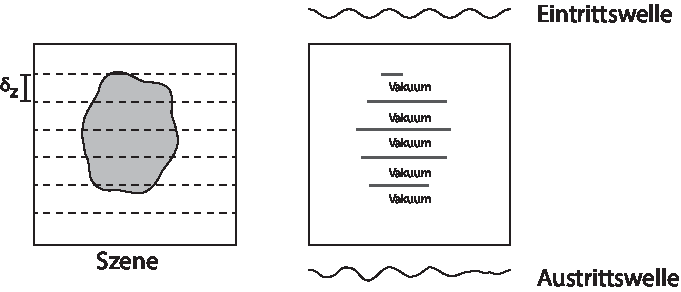
\includegraphics[width=0.9\textwidth]{images/multislice.pdf}
	\caption[Prinzip Multislice Propagation]{Prinzip Multislice Propagation: Die Szene wird in einzelne Schichten zerlegt und die Wechselwirkung mit der Materie jeder einzelnen Schicht in auf eine in dieser Schicht liegenden Ebene reduziert. Zwischen diesen Ebenen wird eine Vakuumpropagation angewendet.}
	\label{fig:multislice}
\end{figure} 	

Bei diesem Verfahren wird die Annahme getroffen, dass  innerhalb einer Schicht die örtliche Verteilung der Materie konstant ist, sowie die durch die Propagation bedingte Veränderung innerhalb von $\Delta z$ ausreichend klein ist, sodass keine Anteile der Wellenfront innerhalb einer Schicht unterschiedliche Brechzahlen durchlaufen \cite{hare1994}. Dies kann durch ein hinreichend kleines $\Delta z$ gewährleistet werden. 
Des Weiteren wird bei der Wechselwirkung mit der Materie der Winkel mit dem ein Anteil der Wellenfront durch die Materie läuft vernachlässigt: Bei Anteilen der Welle, die durch vorangegangene Streueffekte bereits in einem deutlichen Winkel die Szene durchlaufen wird genähert, dass ihr Weg durch die Materie gleich lang wie der Weg von nicht gestreuten Anteilen ist. Somit wird Mehrfachstreuung zwar mitberücksichtigt, jedoch nur näherungsweise.
	
Der Algorithmus zur Berechnung der Austrittswelle lautet somit
\begin{equation}
	\label{eq:multislice}
	\Phi(z+\Delta z)= e^{i\delta n\left(z\right) \Delta z}\mathscr{F}^{-1}\left[e^{i\Delta z\sqrt{k^2-(q_x+q_y)^2}}\mathscr{F}\left[\Phi(z)\right]\right]
\end{equation}
Ist die Austrittswelle bekannt, so ist die weitere Ausbreitung zum Detektor eine Vakuumpropagation, die sich entweder mittels Angular Spectrum Propagation berechnen lässt, oder sich durch eine einfache Fouriertransformation in Fraunhofer-Näherung bestimmen lässt. Ersteres Verfahren hat den Nachteil, das es bei einer numerischen Implementation im Bereich der Szene die gleiche räumliche Rastergröße wie im Bereich des Detektors erfordert, während bei Anwendung der Fernfeld Näherung zwar der maximale Winkel in dem das Streubild berechnet werden kann von der räumlichen Auflösung der Austrittswelle sowie die Winkelauflösung von der Szenenausdehnung abhängt, dies jedoch deutlich praktikabler ist.
Diese Methode wird im Weiteren als \textit{Multislice Propagation} bezeichnet und ist in \texttt{simulation/multislice.m} implementiert.
	
\section{Thibaults Multislice}
Thibault stellt in \cite{thibault2007} einen eigene Formulierung der Multislice-Simulation auf. Ausgehend von der Wellengleichung
lässt sich für die Welle im Hybridraum
\begin{equation}
	\tilde{\Phi}(z)=\tilde{G}\ast_z\left[\tilde{\delta\eta}\ast_{q_\perp} \tilde{\Phi}\right]
\end{equation}
mit
\begin{equation}
	\tilde{G}=\frac{1}{2\pi}\frac{ik^2}{\sqrt{k^2-q_\perp^2}}e^{iz(\kappa-k)}
\end{equation}
aufstellen. Hierbei sind die Faltungsoperatoren mit den Variablen über die die Faltung durchzuführen ist indiziert.
Wird nun die Welle bei $\Delta z$ betrachtet, so lässt sich unter Vernachlässigung von Rückstreuung  das Faltungsintegral über $z$ in zwei Integrationsbereiche aufspalten (vom Ursprung bis $\Delta z$ sowie von dort bis ins Unendliche):
\begin{equation}
	\tilde{\Phi}(z+\Delta z)=
	\int_{\Delta z}^{\infty} \tilde{G}(z')\left[\tilde{\delta\eta}\ast_{q_\perp} \tilde{\Phi}\right](z+\Delta z-z')\dif z'
	+
	\int_{0}^{\Delta z} \tilde{G}(z')\left[\tilde{\delta\eta}\ast_{q_\perp} \tilde{\Phi}\right](z+\Delta z-z')\dif z'
\end{equation}
Für den ersten Summanden gilt mit einer Substitution ($z'\rightarrow z''+\Delta z$)
\begin{align*}
	  & \stackrel{\hphantom{z'\rightarrow z''+\Delta z}}{\hphantom{=}} 
	\int_{\Delta z}^{\infty} \tilde{G}(z')\left[\tilde{\delta\eta}\ast_{q_\perp} \tilde{\Phi}\right](z+\Delta z-z')\dif z'\\
	  & \stackrel{z'\rightarrow z''+\Delta z}{=}                       
	\int_{0}^{\infty} \tilde{G}(z''+\Delta z)\left[\tilde{\delta\eta}\ast_{q_\perp} \tilde{\Phi}\right](z-z'')\dif z''\\
	  & \stackrel{\hphantom{z'\rightarrow z''+\Delta z}}{=}            
	e^{i\Delta z(\kappa-k)}\int_{0}^{\infty} \frac{1}{2\pi}\frac{ik^2}{\sqrt{k^2-q^2_\perp}}e^{iz''(\kappa-k)}\left[\tilde{\delta\eta}\ast_{q_\perp} \tilde{\Phi}\right](z-z'')\dif z''\\
	  & \stackrel{\hphantom{z'\rightarrow z''+\Delta z}}{=}            
	e^{i\Delta z(\kappa-k)}\tilde{\Phi}(z) \numberthis \,,
\end{align*}
im zweiten Summanden kann für hinreichend kleine $\Delta z$ das Integral gut durch eine Rieman-Obersumme mit einem einzigen Stützpunkt bei $\Delta z$ approximiert werden:
\begin{equation}
	\int_{0}^{\Delta z} \tilde{G}(z')\left[\tilde{\delta\eta}\ast_{q_\perp} \tilde{\Phi}\right](z+\Delta z-z')\dif z'
	\approx
	\Delta z \tilde{G}(\Delta z)\left[\tilde{\delta\eta}\ast_{q_\perp} \tilde{\Phi}\right](z)
\end{equation}
Für den Fehler dieser Näherung gilt
\begin{equation}
	\text{Rieman AbschätzungXX}
\end{equation}
Somit lässt sich in Näherung für die Welle bei $z+\Delta z$
\begin{equation}
	\label{eq:thibault}
	\tilde{\Phi}(z+\Delta z)
	\approx
	e^{i\Delta z(\kappa-k)}
	\left(
	\tilde{\Phi}(z)+\frac{\Delta z}{2\pi}\frac{ik^2}{\sqrt{k^2-q^2_\perp}}  \left[\tilde{\delta\eta}\ast_{q_\perp} \tilde{\Phi}\right](z)
	\right)
\end{equation}
aufstellen. Dies stellt einer iterative Beschreibung der Streuung dar --- ausgehend von $z=0$ kann schrittweise in Einfallsrichtung die Wellengleichung in einer Szene gelöst werden. Somit handelt es sich um ein Algorithmus der ebenfalls der Kategorie "`Multislice"' zuzuordnen ist. Im Gegensatz zur \textit{Multislice Propagation} findet hier die Wechselwirkung mit der Materie jedoch nicht in Form eines Exponentialfaktor statt, in Kleinwinkelnäherung entspricht \fref{eq:thibault} einer Taylornäherung erster Ordnung in der Exponentialfunktion von \fref{eq:multislice}. Unabhängig von der Gültigkeit der verwendeten Näherungen besitzt \eqref{eq:thibault} bei $k^2=q_\perp$ eine Singularität. Aus diesem Grund muss entweder das Raster in dem die Simulation durchgeführt hinsichtlich der Auflösung in x,y-Richtung so gewählt werden, dass diese Singularität nicht zu tragen kommt oder nach jedem Simulationsschritt im Fourierraum $\tilde{\Phi}(q_x,q_y)$ für $q_x+q_y>k$ auf Null gesetzt werden.
Die numerische Simulation dieser Methode ist in \texttt{simulation/thibault.m} implementiert.


\section{Verifizierung}
Zur Verifizierung der vorgestellten Simulationsalgorithmen und deren numerische Implementierungen eignet sich der Vergleich der berechneten Streubilder hinter Kugeln mit den Ergebnissen aus der Berechnung mittels Mie-Streuung. Der Vergleich wird für verschiedene Brechzahlen und Kugelradien bei einer Wellenlänge von 1\si{nm} durchgeführt.

Da ein realer Detektor nicht die Intensitäten bei präzise definierten Winkelpunkten misst sondern innerhalb eines Areals, ist es zweckmäßig, die simulierte Detektorfläche in quadratische Areale zu unterteilen und die Intensität in jedem dieser Areale als gewichtetes Mittel zwischen in dem Areal liegenden Punkten zu betrachten.
Hierbei werden an den Rändern zwischen zwei Arealen liegende Berechnungspunkte zur je zur Hälfte in beiden Arealen, in der Ecke zwischen vier Arealen liegende Berechnungspunkte je zu einem Viertel in den vier Arealen berücksichtigt.
Besonders bemerkbar ist dieser Bearbeitungsschritt bei Pixeln die genau in den Intensitätsminima liegen: Ohne die gewichtete Mittlung würde der gesamten Fläche zwischen den Pixeln die Intensität des Minimums zugewiesen werden, auch wenn dessen Breite extrem schmal ist, werden zusätzliche Pixel berechnet und anschließend gewichtet gemittelt, ergibt sich eine korrektere Wiedergabe des tatsächlichen Intensitätsverlaufs (\fref{fig:average}). Dies wird sowohl für die mit den verschiedenen Algorithmen simulierten Streubildern als auch für die Mie-Streubilder durchgeführt.

Anschließend werden die simulierten Streubilder bezüglich ihrer Skalierung auf die Mie-Streubilder normiert. Hierzu wird ein Skalierungsfaktor gesucht, der die mittlere Abweichung der simulierten Streubilder vom jeweiligen Mie-Streubild innerhalb der ersten 10° minimiert. Zur Quantifizierung des Fehlers der simulierten Streubilder wird die relative Abweichung von den Mie-Streubildern betrachtet.
Die relative Abweichung von Mie ist für einen konkreten Parametersatz exemplarisch dargestellt in \fref{fig:relerror}. Aus den rotationssymmetrischen Streubildern können Radialprofile der Intensität sowie des relativen Fehlers bestimmt werden um einen besseren Überblick zu erhalten. \fref{fig:profil}).
Es ist zu erkennen, dass der relative Fehler in den Datenpunkten, in denen das Mie-Profil ein Minimum hat, aufgrund des steilen Verlaufs scharfe, nur 1-2 Datenpunkte umfassende, Maxima annimmt.
Um eine quantifizierende Größe für die Güte einer Simulation bei einem bestimmten Radius und Stoffeigenschaften zu haben, wird deshalb der Median des relativen Fehlers bis 20° Streuwinkel genutzt. So ist es möglich, für die unterschiedlichen Simulationsalgorithmen Bereiche zu bestimmen, in denen sie ausreichend mit der Mie-Theorie übereinstimmen, um sie als in diesem Bereich valide anzusehen \fref{fig:variation}. Es ist zu erkennen dass bei Werten von $\delta$ bzw. $\beta$ in der Größenordnung bis $10^{-4}$ die viele Materialien bei 1\si{nm} Wellenlänge aufweisen \cite{henke} sowohl \textit{Multislice Propagation} und\textit{ Thibaults Multislice} als auch \textit{MSFT} valide Ergebnisse liefern --- der mediane Fehler überschreitet 5\% nicht. Bei größeren Abweichungen der Brechzahl von der Vakuumbrechzahl steigt der mediane Fehler des mittels \textit{MSFT} berechneten Streubildes deutlich an, insbesondere bei großen Radien. Bei diesen kommt es zu deutlich mehr Mehrfachstreuung in Vorwärtsrichtung, die bei \textit{MSFT} im Gegensatz zu den beiden anderen Multislice Varianten vollständig ignoriert wird. Der Unterschied zwischen Thibaults Formulierung und der \textit{Multislice Propagation} kann zu einem gewissen Anteil durch die verwendete naive Implementierung von Thibaults Algorithmus begründet sein. Hier besteht weiteres Optimierungspotential bezüglich der numerischen Genauigkeit und dem Einfluss von Rundungsfehlern.


\begin{figure} %mittelwert
	\centering
	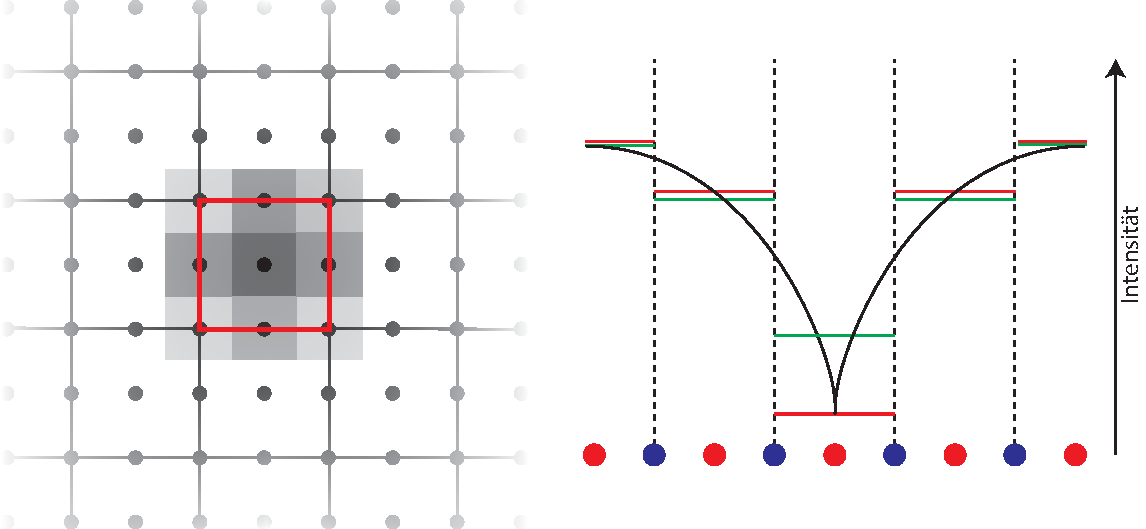
\includegraphics[width=0.9\textwidth]{images/average.pdf}
	\caption[Gewichteter Mittelwert]{Die Verwendung von Überabtastung und gewichteten Mittelwertes bei den Streubildern: Um die Intensität im links rot umrandeten Bereich zu bestimmen, wird die Intensität an den Schwarzen Punkten berechnet und ein gewichteter Mittelwert gebildet, indem die Intensität der vier Randwerte zur Hälfte, die der vier Eckpixel zu einem Viertel in dem umrandeten Bereich mitberücksichtigt werden. Der Effekt gegenüber einer Berechnung nur in den Zentren der Pixel zeigt sich rechts: Wird die Intensität bei einem schwarz dargestellten wahren Intensitätsverlauf nur an den roten Punkten bestimmt, dominiert das Minimum den Intensitätsverlauf. Eine geringere Abweichung ergibt sich bei Berechnung auch an den blauen Punkten und Bildung des gewichteten Mittelwert (grün).}
	\label{fig:average}
\end{figure} 




\begin{figure} %exitwave und scatter
	\centering
	\begin{subfigure}[b]{0.49\textwidth}
		\setbox1=\hbox{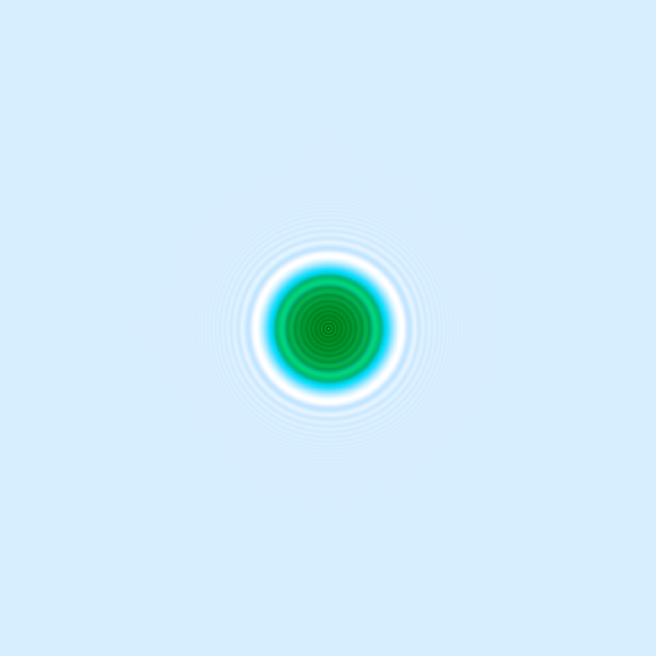
\includegraphics[width=\textwidth]{images/fig_sim_exitwave_multislice-r100-bd1e-3.png}}
		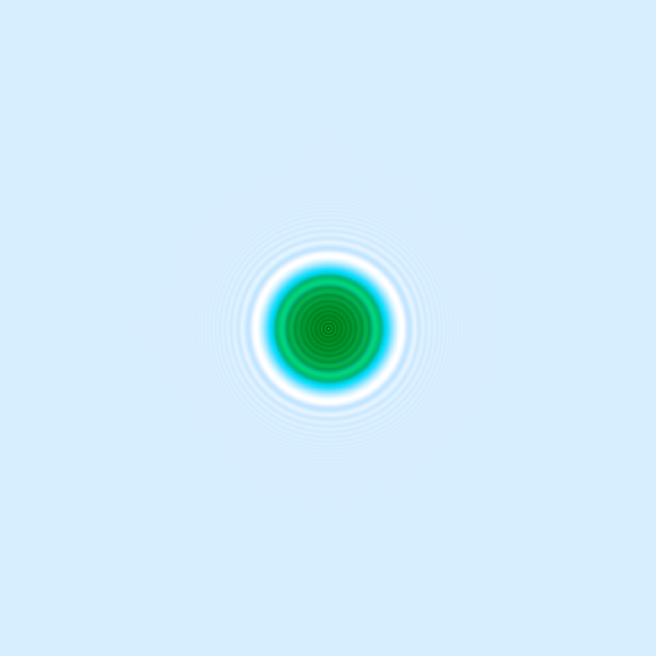
\includegraphics[width=\textwidth]{images/fig_sim_exitwave_multislice-r100-bd1e-3.png}\llap{\makebox[\wd1][l]{\includegraphics[width=0.5\textwidth]{images/fig_sim_exitwave_multislice_cw-r100-bd1e-3.pdf}}}
				  
		\caption{Austrittswelle}
		\label{fig:exitwave}
	\end{subfigure}
	\begin{subfigure}[b]{0.49\textwidth}
		\setbox1=\hbox{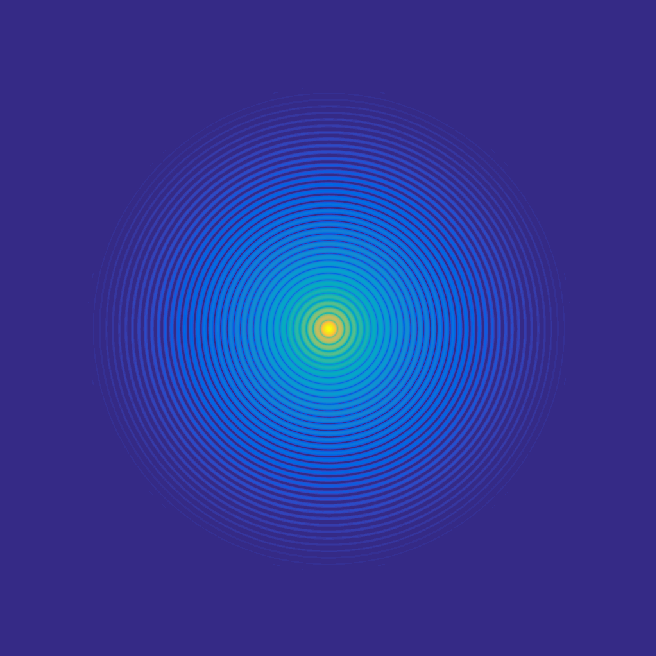
\includegraphics[width=\textwidth]{images/fig_sim_scatter_multislice-r100-bd1e-3.png}}
		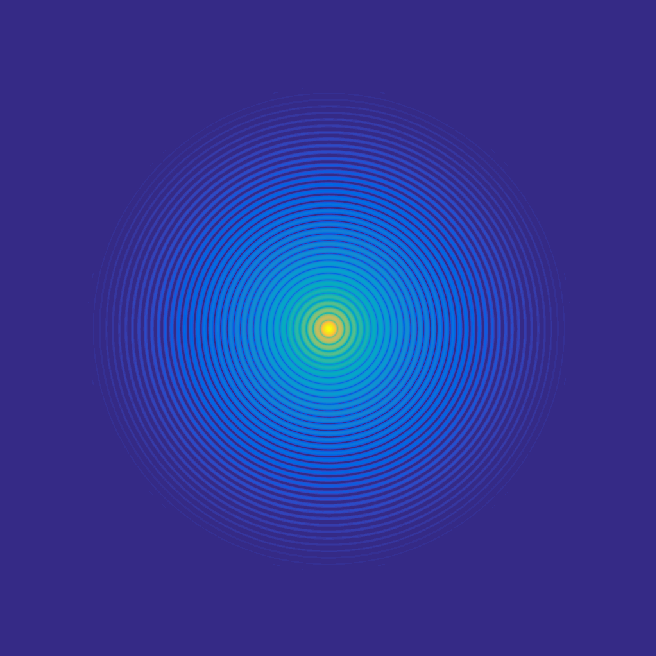
\includegraphics[width=\textwidth]{images/fig_sim_scatter_multislice-r100-bd1e-3.png}\llap{\makebox[\wd1][l]{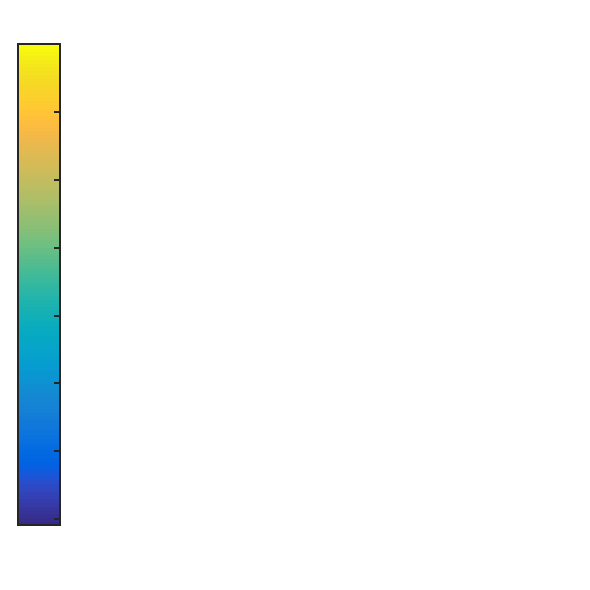
\includegraphics[width=0.5\textwidth]{images/fig_sim_scatter_multislice_cb-r100-bd1e-3.pdf}}}
		\caption{Streubild}
		\label{fig:scatter}
	\end{subfigure}
	\caption[Austrittswelle und Streubild einer Kugel]{Exemplarische Multislice-Propagations Austrittwelle und (logarithmiertes) Streubild einer Kugel mit Radius 100\si{nm} bei $\beta,\delta$=$10^{-3}$. Die relative Intensität der Austrittswelle bezüglich der Eintrittswelle ist über die Helligkeit dargestellt, die Phase über den Farbton. Das Streubild zeigt einen Bereich bis 15°.}
	\label{fig:exitscatter}
\end{figure}


\begin{figure} %rel error
	\centering
	\begin{subfigure}[b]{0.49\textwidth}
		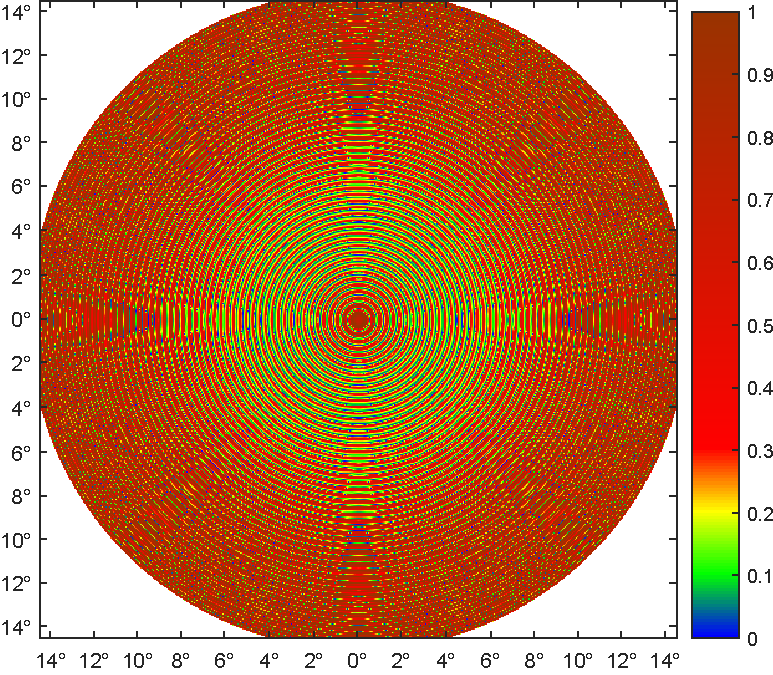
\includegraphics[width=\textwidth]{images/fig_sim_relerror_FTproj-r100-bd1e-3.pdf}
		\caption{Projektion}
	\end{subfigure}
	\begin{subfigure}[b]{0.49\textwidth}
		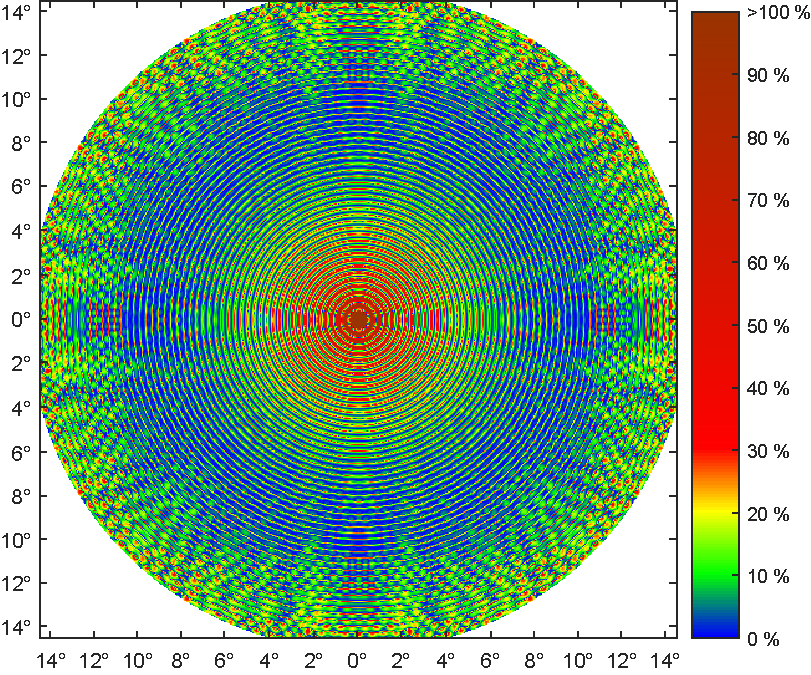
\includegraphics[width=\textwidth]{images/fig_sim_relerror_msft-r100-bd1e-3.pdf}
		\caption{MSFT}
	\end{subfigure}
	%	\par\bigskip
	\begin{subfigure}[b]{0.49\textwidth}
		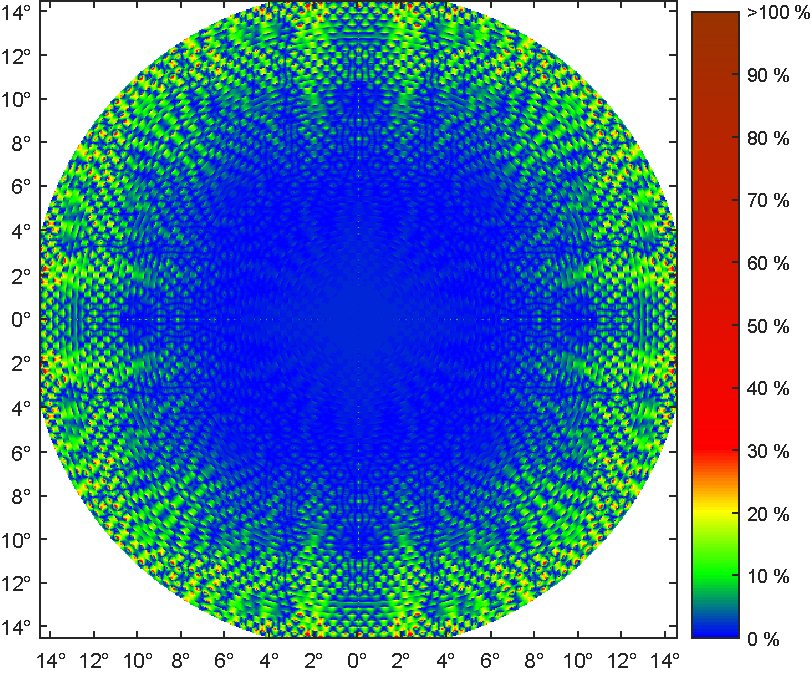
\includegraphics[width=\textwidth]{images/fig_sim_relerror_thibault-r100-bd1e-3.pdf}
		\caption{Thibaults Multislice}
	\end{subfigure}
	\begin{subfigure}[b]{0.49\textwidth}
		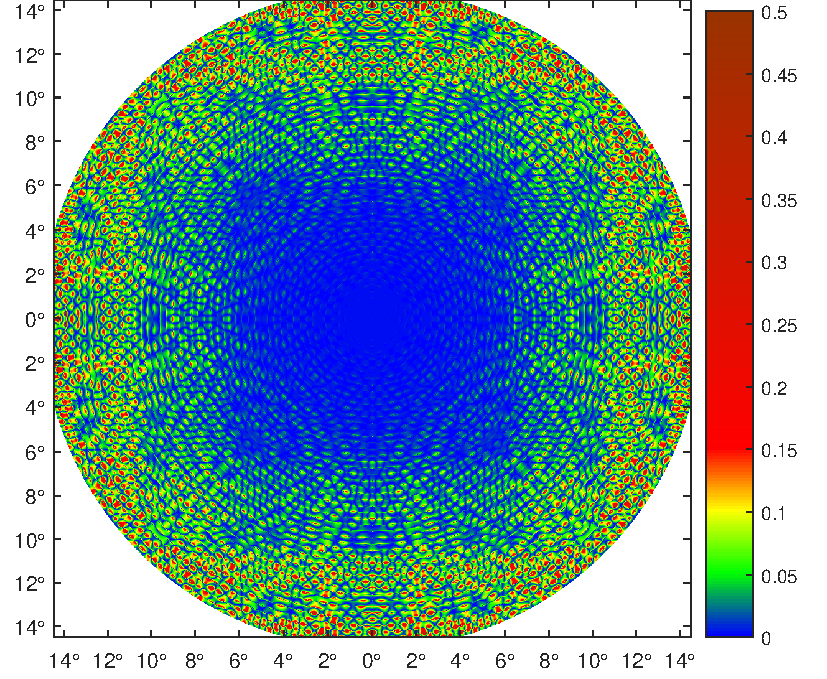
\includegraphics[width=\textwidth]{images/fig_sim_relerror_multislice-r100-bd1e-3.pdf}
		\caption{Multislice Propagation}
	\end{subfigure}
		
	\caption[relativer Fehler der Simulationen]{Relative Abweichungen von Mie der simulierten Streubilder einer Kugel mit Radius 100\si{nm} bei $\beta=\delta=10^{-3}$. }
	\label{fig:relerror}
\end{figure}
\begin{figure} %profile
	\centering
	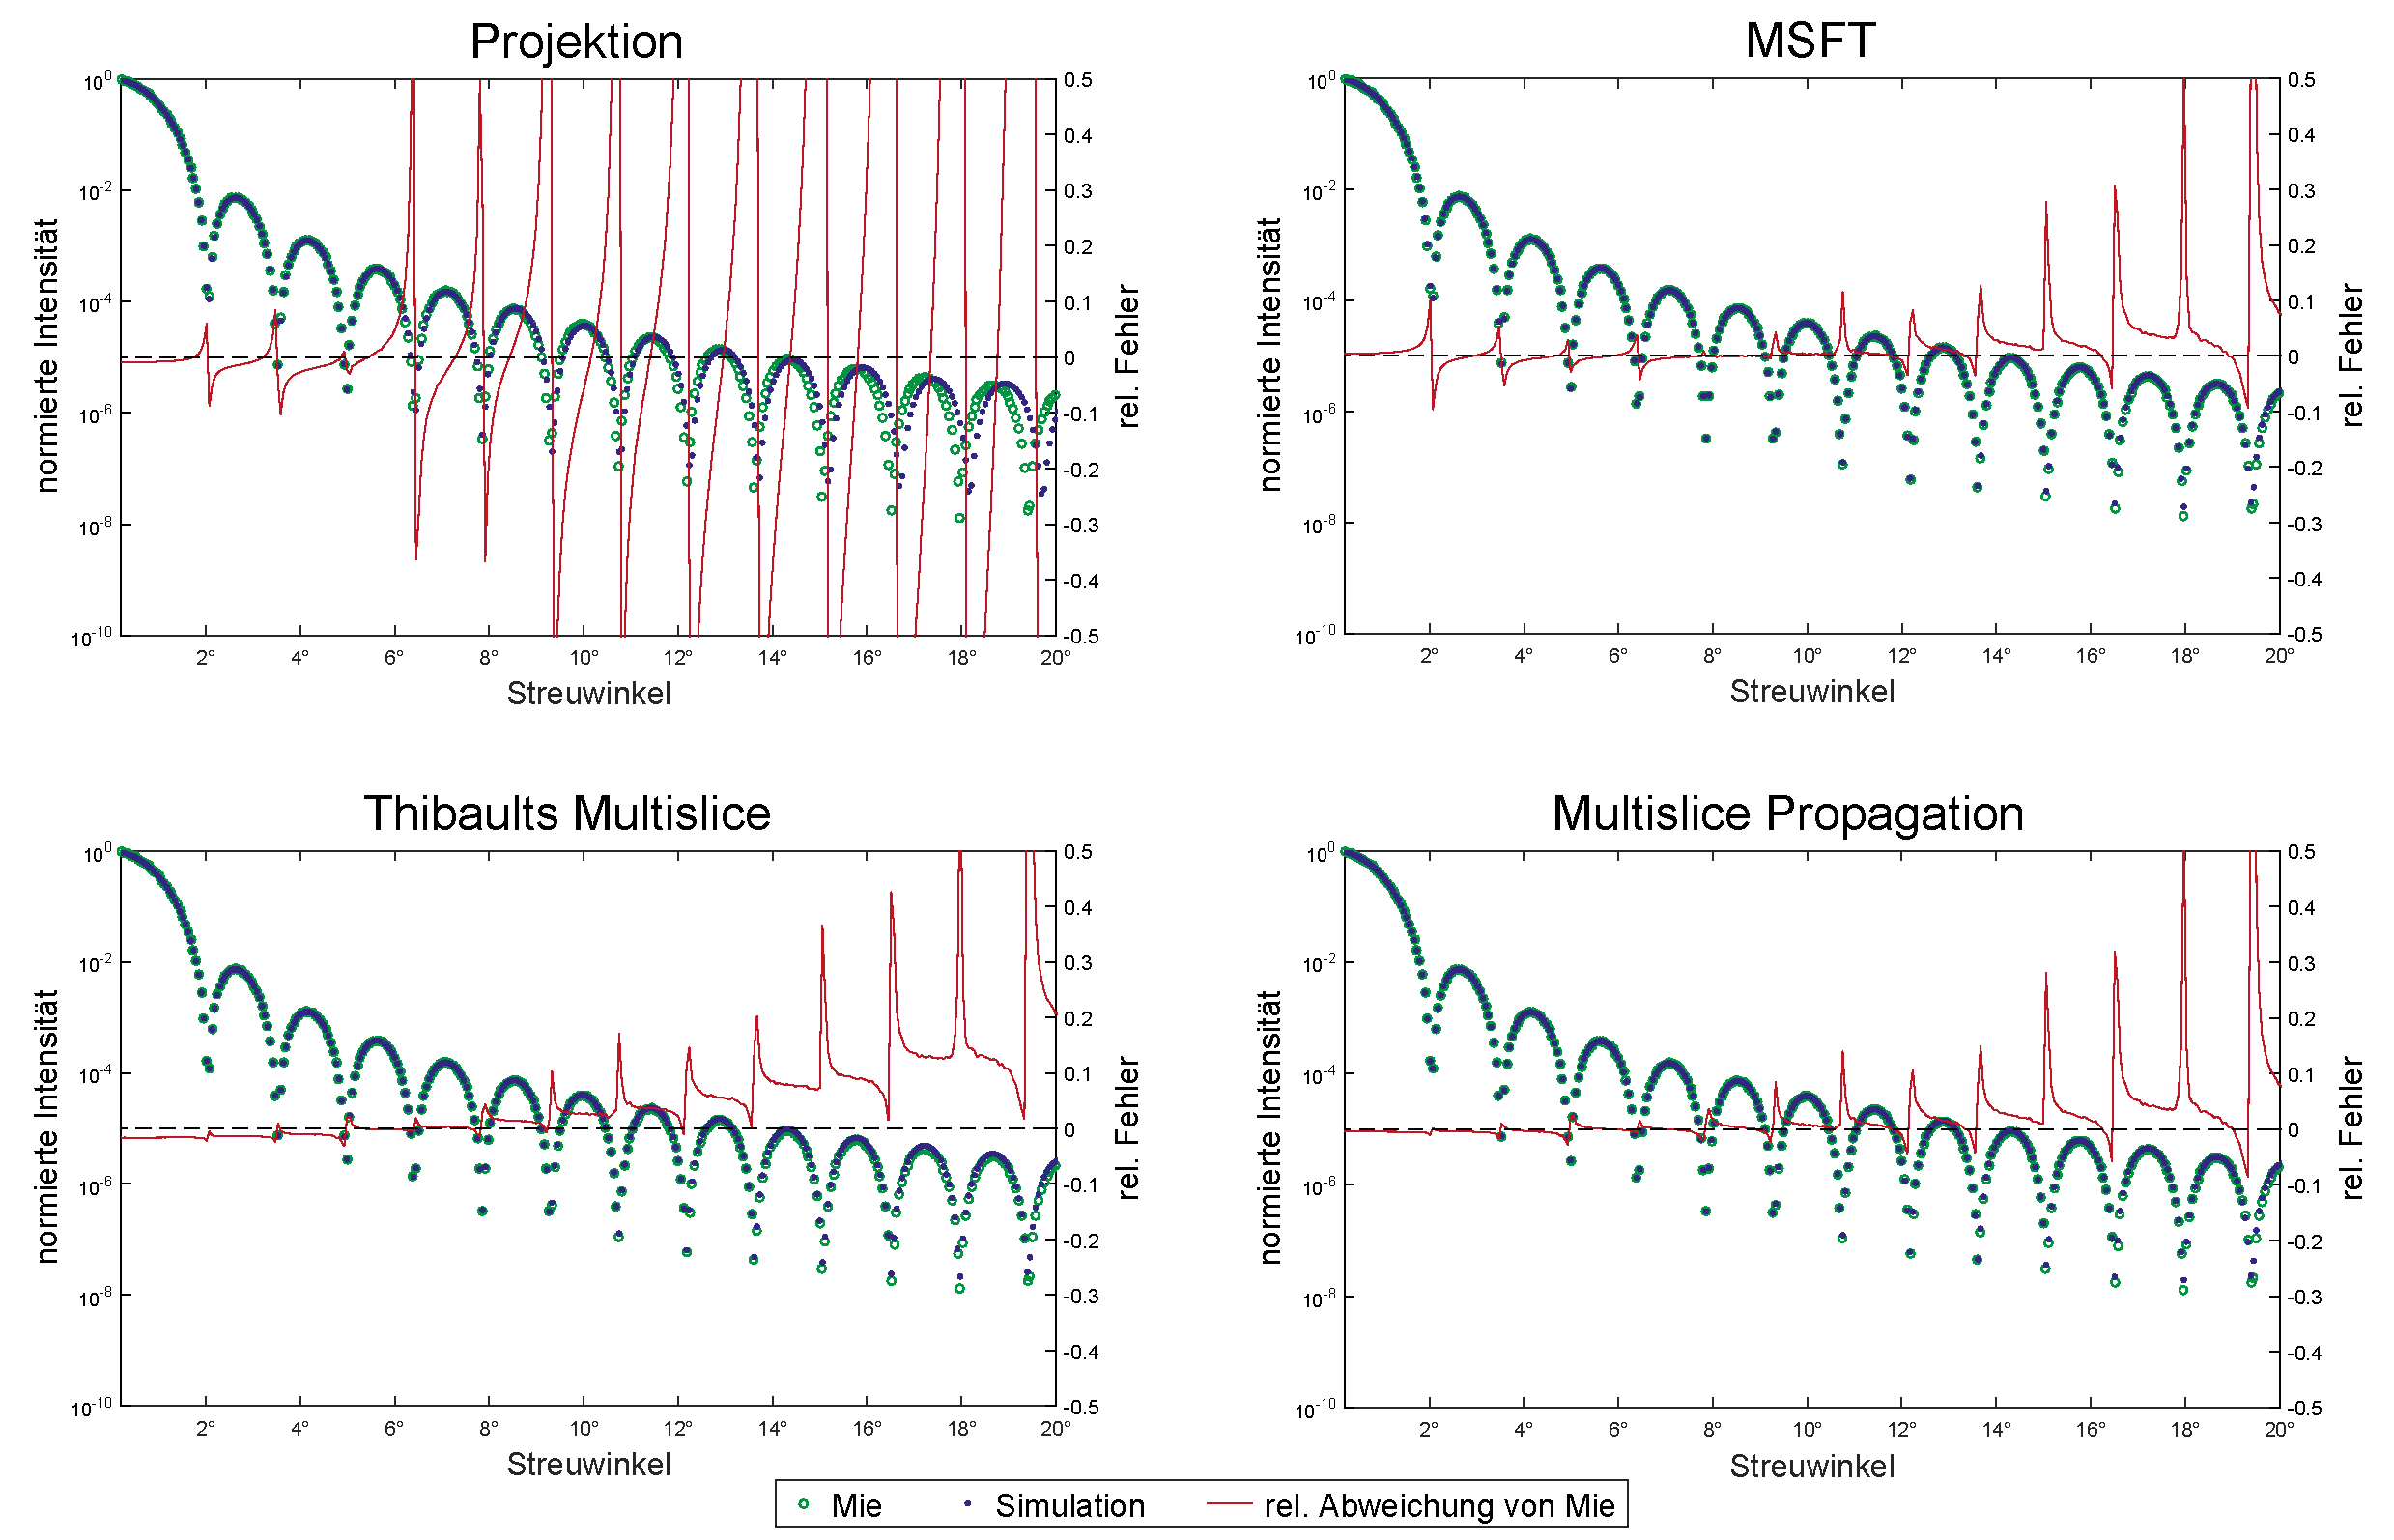
\includegraphics[width=1\textwidth,trim=60 5 30 10,clip]{images/fig_sim_profile.pdf}
	\caption[Radiale Profile]{Radiale logarithmierte Intensitätsprofile berechnet mit den verschiedenen Algorithmen sowie die relative Abweichung von Mie für eine Kugel mit Radius 20 \si{nm} und $\beta,\delta$=$10^{-4}$. Es ist bei kleinen Streuwinkeln eine gute Übereinstimmung aller Algorithmen zu erkennen, bei höheren Winkeln versagt die Projektion. Über den gesamten Bereich besitzt bei diesen Parametern die Multislice Propagation die beste Übereinstimmung. Die relativen Fehler der Simulationen besitzen in den Intensitätsminima aufgrund der dort deutlich Abfallenden Referenzintensität deutliche Maxima.}
	\label{fig:profil}
\end{figure}

\begin{figure} %parameter variation
	\centering
	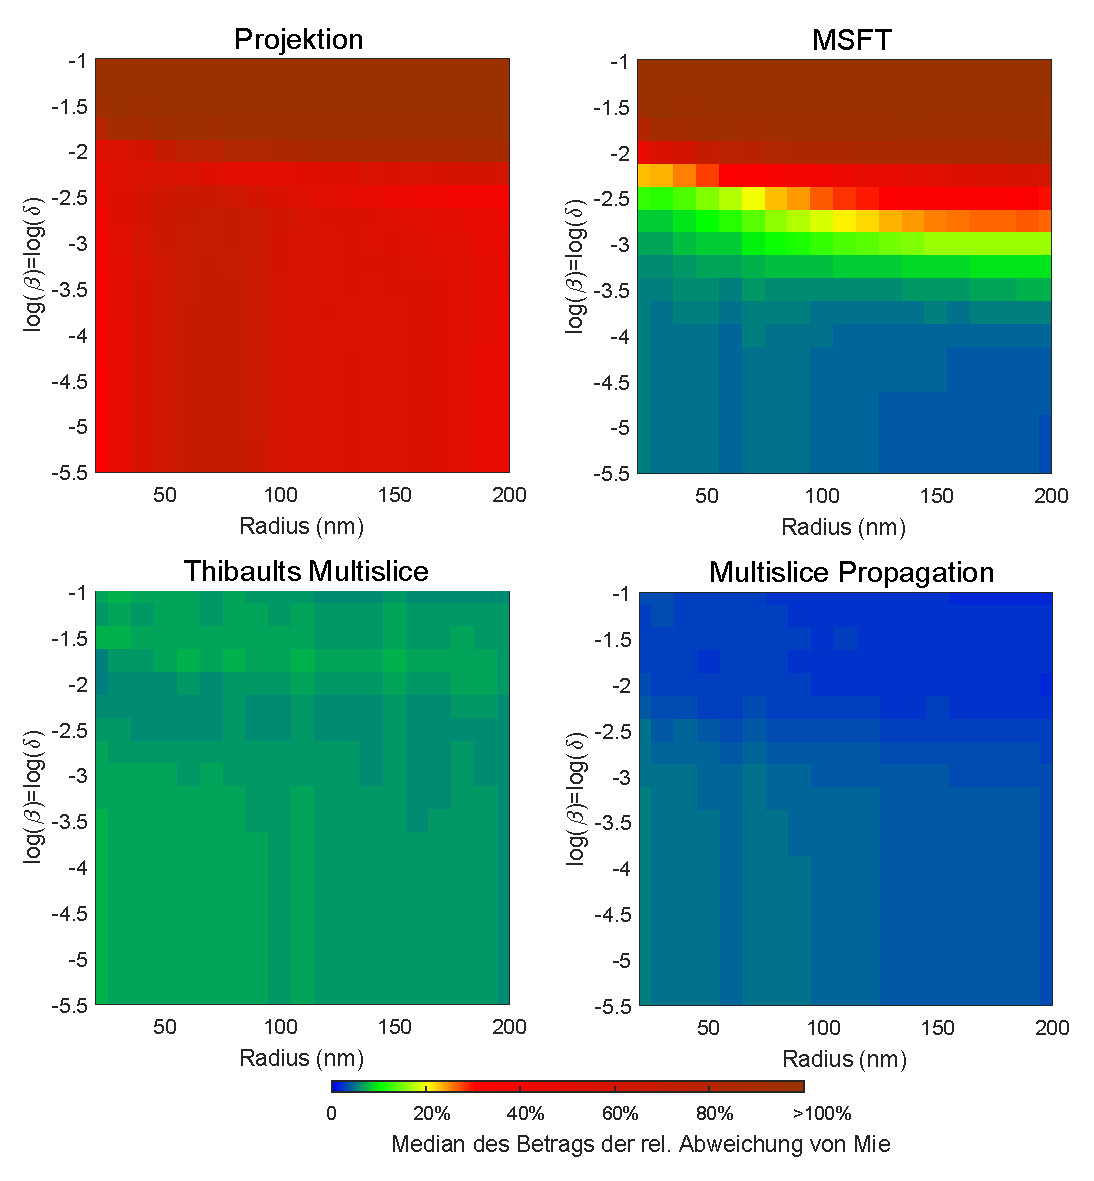
\includegraphics[width=1\textwidth]{images/fig_sim_var.pdf}
	\caption[Gültigkeit der Simulationsalgorithmen]{Zur Entscheidung bei welchen Radien und welchen Abweichung der Brechzahl vom Vakuum die Simulationen noch valide sind, ist die mediane, relative Abweichung bis 20° von Mie über den Parametern aufgetragen. Es somit die Bereiche erkennbar, in denen der jeweilige Simulationsalgorithmus valide Ergebnisse liefert. Parameter: $\Delta x=\sfrac{\lambda}{2}$, $\Delta z$ als $\sfrac{\lambda}{8}$ und N=2048.}
	\label{fig:variation}
\end{figure}



\section{Streubilder komplexer Objekte}
Neben der Berechnung von Streubilder von Kugeln eignen sich die Simulationsalgorithmen auch zur Berechnung der Austrittswellen und Streubilder hinter anderen Objekten.

Als interessante Testszene wird eine wassergefüllte ikosaederförmige Lecithin-Membran mit dem Außenradius 375 \si{nm} und einer Dicke von 25 \si{nm} um deren Mittelpunkt vier kleinere, DNA gefüllte Kugeln (Radius 90 \si{nm}) in den Eckpunkten eines Tetraeders angeordnet sind (\fref{fig:komplexmodel}) sowie ein disjunktes Xenon-Dodekaeder mit Außenradius 100 \si{nm} betrachtet. Die komplexen Brechzahlen sind in \fref{tab:brechzahl} aufgeführt \cite{henke,bergh2008,milo2015}. Die so berechnete Austrittswelle ist in \fref{fig:komplexexit} dargestellt, das zugehörige Streubild ist in \fref{fig:komplexscatter} und stellt das Ergebnis der Bemühungen synthetische Streubilder zu erstellen dar und lässt sich für den Vergleich von Rekonstruktionsansätzen nutzen.

  
\begin{table}
	\begin{minipage}[b]{.64\textwidth }%
	 	\begin{small}
 			\begin{tabular}{lll}
 				\hline
 				Material													&Brechzahl bei 1 \si{nm} \cite{henke}\\
 				\hline
 				Lecithin (\chem{C_{44}H_{82}NO_8P}) \cite{milo2015}			&$1-(1.69-0.12i)\times10^{-4}$			\\ 					
 				Wasser														&$1-(1.55-0.18i)\times10^{-4}$			\\
 				Protein (\chem{H_{86}C_{52}N_{13}O_{15}S}) \cite{bergh2008}	&$1-(2.03-0.16i)\times10^{-4}$			\\
 				Xenon-Cluster												&$1-(2.54-1.46i)\times10^{-4}$			\\
 				\hline
 			\end{tabular}
		\end{small}
		\centering
		\caption[Materialen für komplexe Austrittswelle]{Brechzahlen der Materialien}   \label{tab:brechzahl}
	\end{minipage}
	\begin{minipage}[b]{.35\textwidth}
				\hspace*{0pt}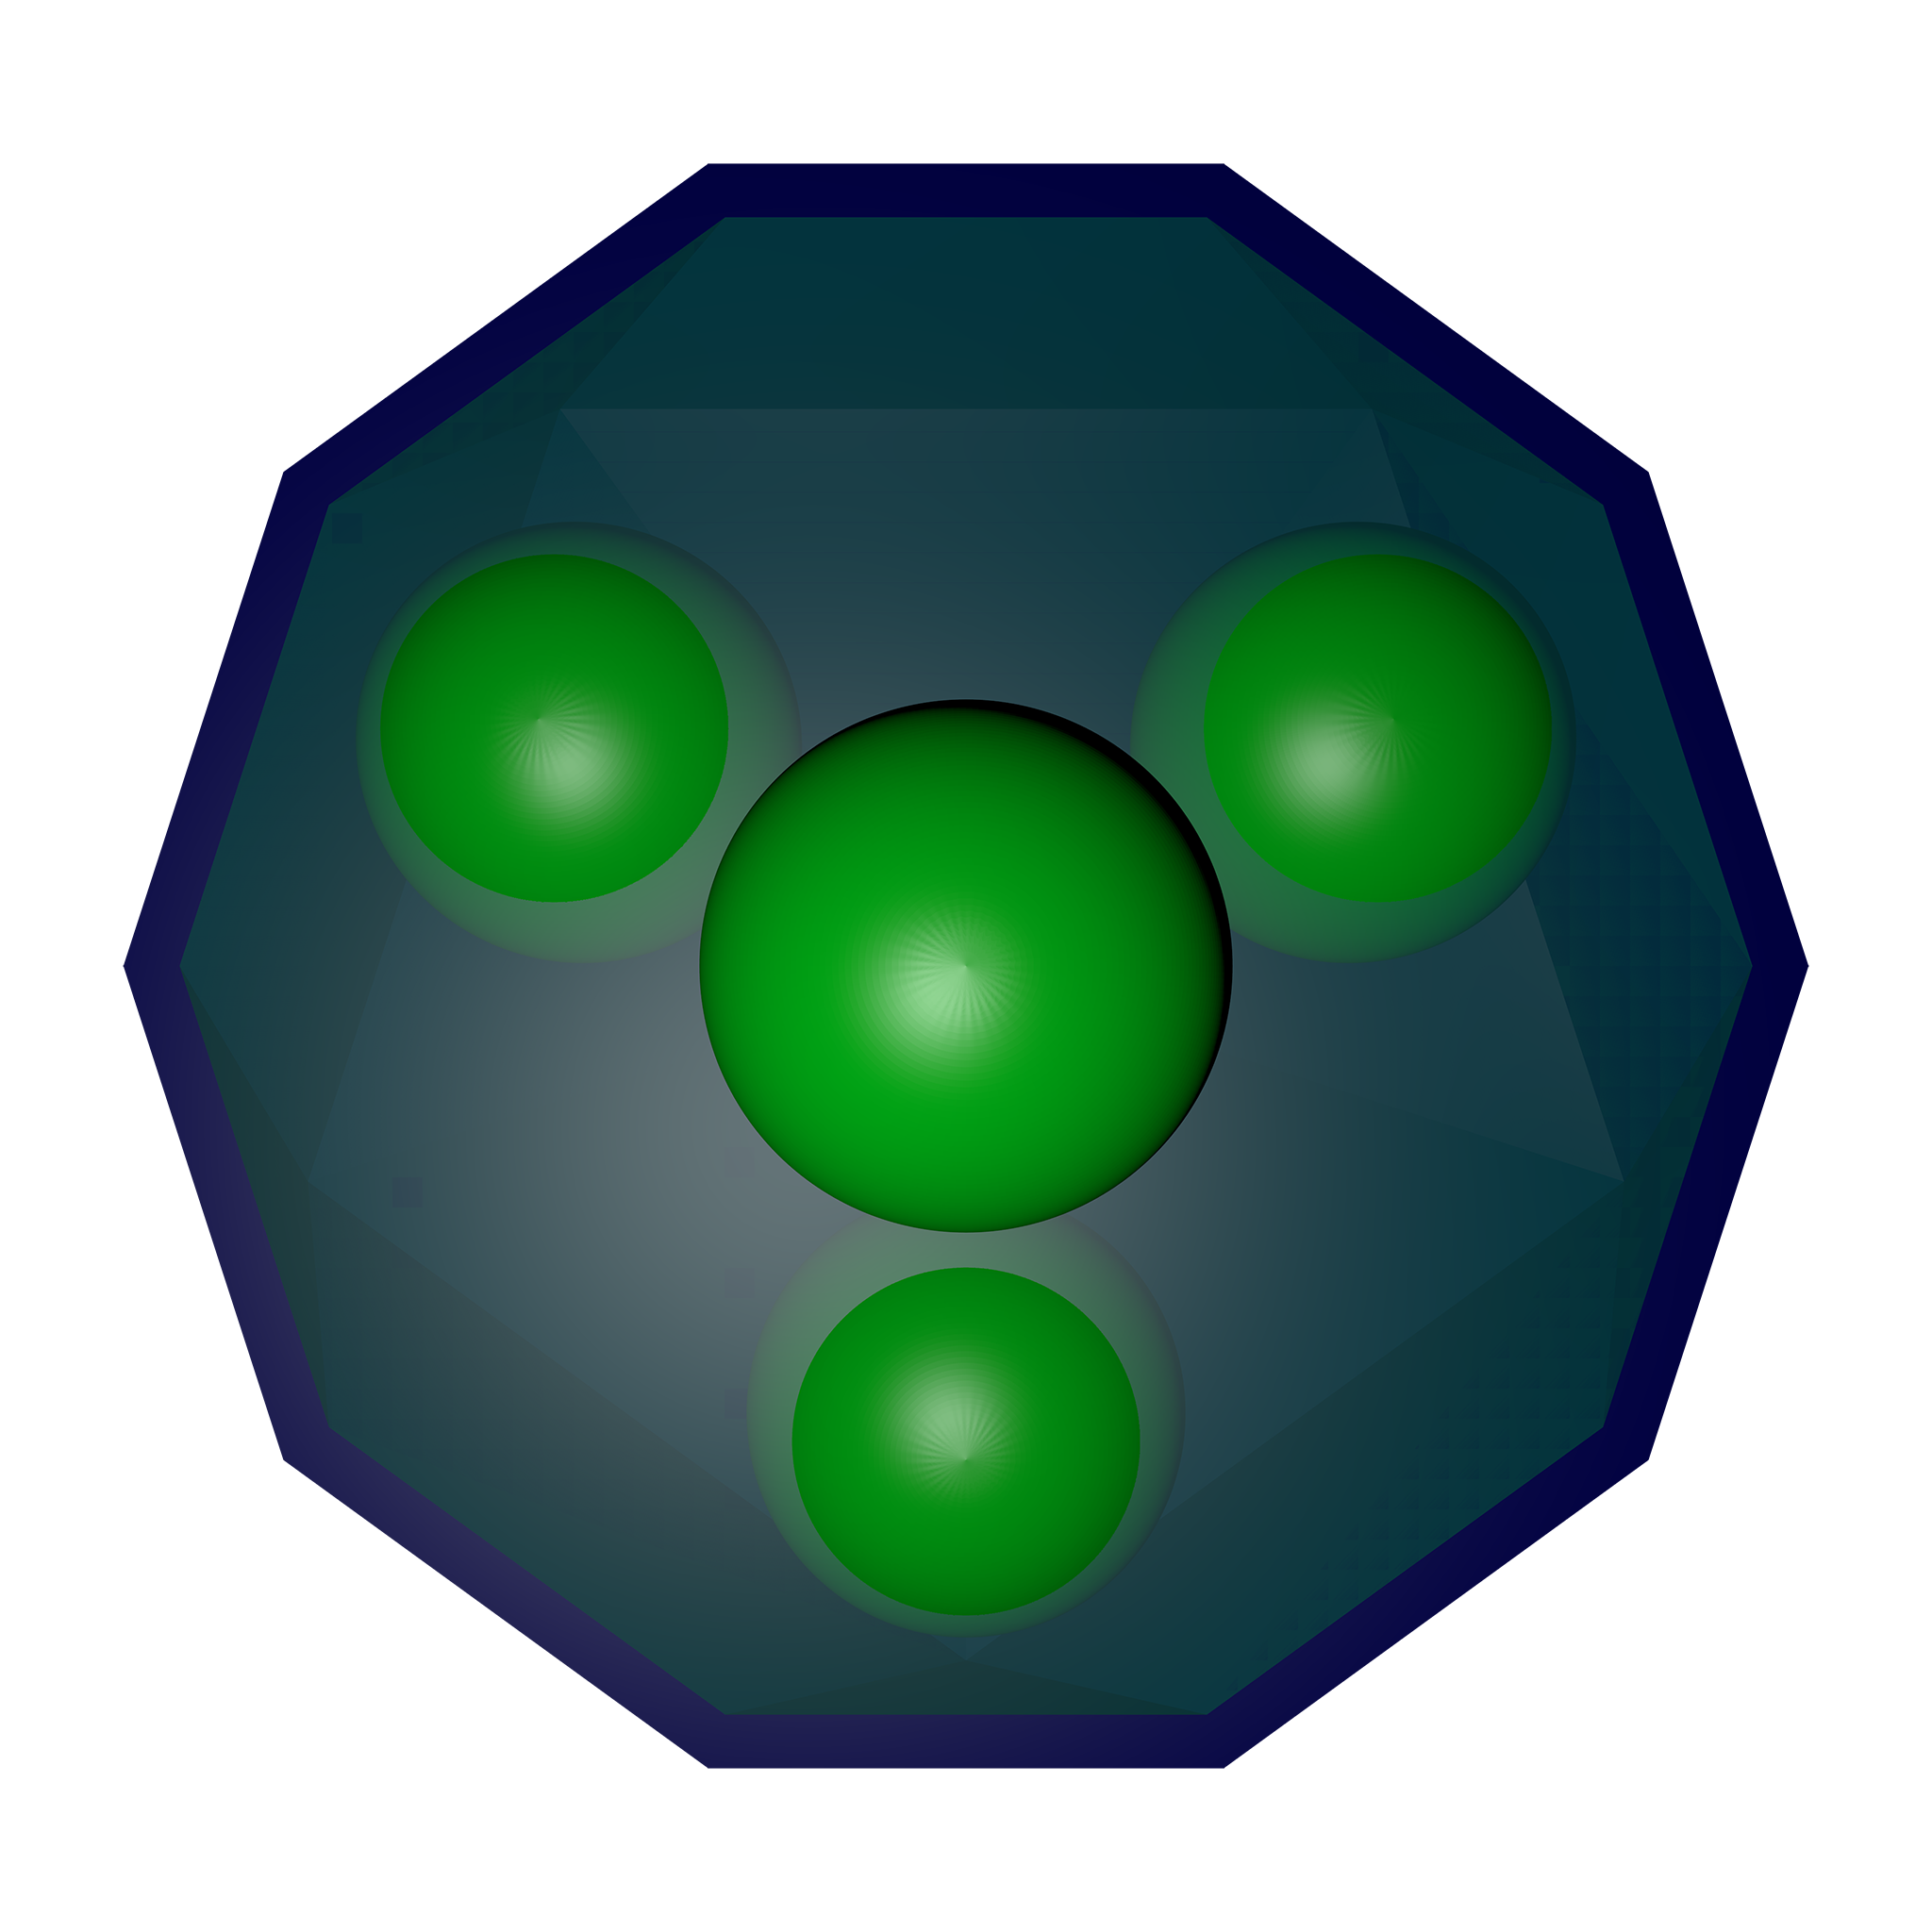
\includegraphics[width=.8\textwidth]{images/scene.png}%
				\captionof{figure}{3D-Modell\label{fig:komplexmodel}}%
	\end{minipage}
\end{table}


\begin{figure} %exitwave und scatter
	\begin{subfigure}[b]{0.49\textwidth}
		\setbox1=\hbox{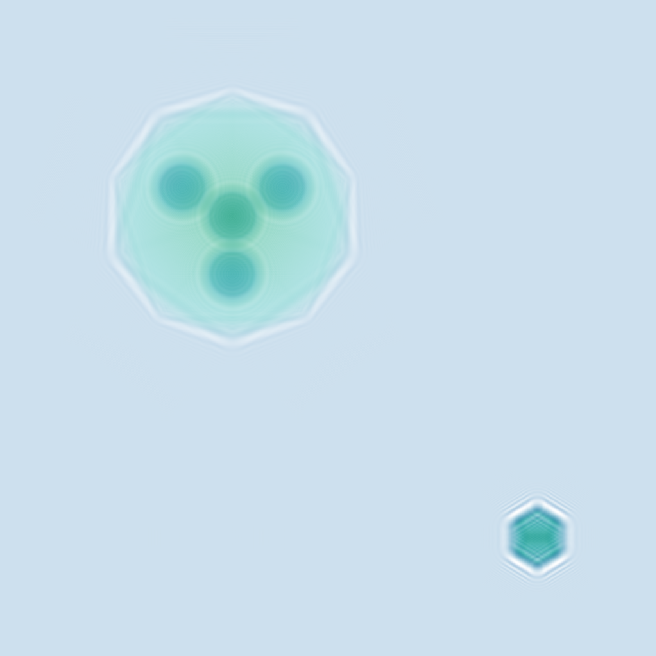
\includegraphics[width=\textwidth]{images/fig_simholo_v2_exitwave.png}}
		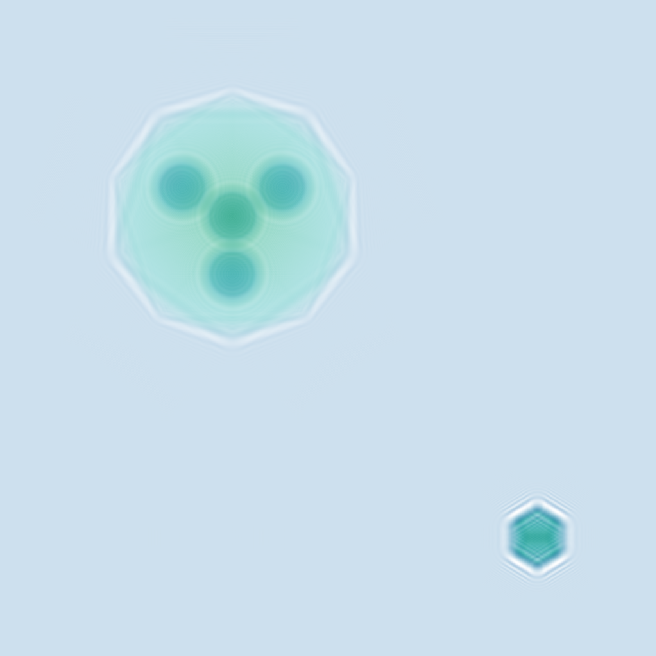
\includegraphics[width=\textwidth]{images/fig_simholo_v2_exitwave.png}\llap{\makebox[\wd1][l]{\includegraphics[width=0.5\textwidth]{images/fig_simholo_v2_exitwave_cw.pdf}}}
		\caption{Austrittswelle}
		\label{fig:komplexexit}
	\end{subfigure}
	\begin{subfigure}[b]{0.49\textwidth}
		\setbox1=\hbox{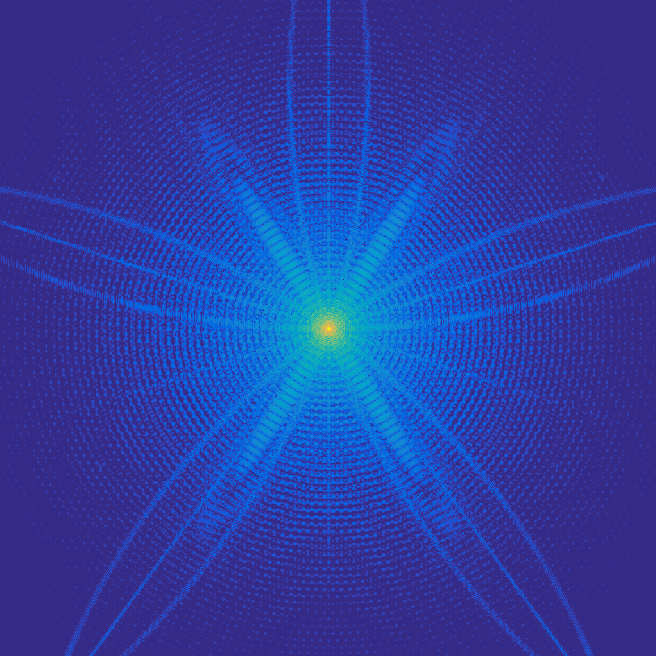
\includegraphics[width=\textwidth]{images/fig_simholo_v2_scatter.png}}
		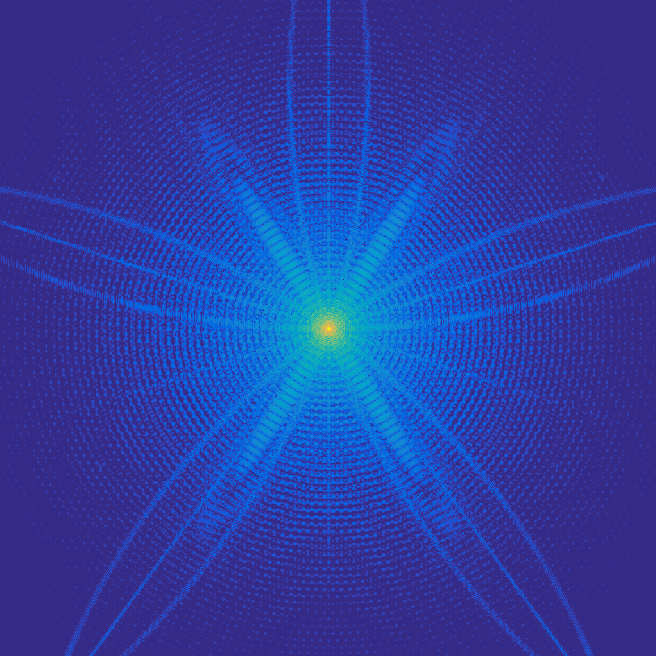
\includegraphics[width=\textwidth]{images/fig_simholo_v2_scatter.png}\llap{\makebox[\wd1][l]{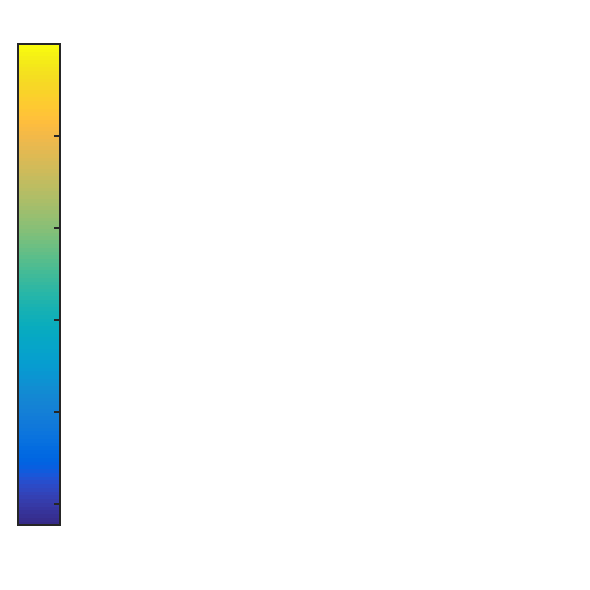
\includegraphics[width=0.5\textwidth]{images/fig_simholo_v2_scatter_cb.pdf}}}
			\caption{Streubild}
			\label{fig:komplexscatter}
	\end{subfigure}		
	\caption[Austrittswelle und Streubild eines komplexen Objektes]{Austrittswelle und logarithmiertes Streubild eines komplexen Objektes. Bei der Austrittswelle ist die relative Intensität bezüglich der Eintrittswelle über die Helligkeit dargestellt, die Phase über den Farbton.}
	\label{fig:komplex}
\end{figure}

